%%%%%%%%%%%%%%%%%%%%%%%%%%%%%%%%%%%%%%%%%%%%%%%%%%%%%%%%%%%%%%%%%%%
\section{Étape 3: Extraction de noyaux et modélisation de leur performance} \label{sec:methodo_step3}
%%%%%%%%%%%%%%%%%%%%%%%%%%%%%%%%%%%%%%%%%%%%%%%%%%%%%%%%%%%%%%%%%%%

Les deux premières étapes de la méthodologie s'intéressent à la recherche et à la caractérisation de nouvelles plateformes. La troisième étape peut être réalisée en parallèle et concerne la modélisation des performances de l'application.


%%%%%%%%%%%%%%%%%
\subsection{Motivations et objectifs}
%%%%%%%%%%%%%%%%%


    En introduction de cette partie, nous avons rappelé la définition des noyaux (\textit{hot spots}). Ceux-ci sont particulièrement présents dans les applications de calcul haute performance qui peut en posséder plusieurs. Ces zones de codes possèdent un fort potentiel pour l'amélioration de la performance de l'application.  Si une application passe 99\% de ses cycles dans l'exécution d'une fonction, une amélioration d'un facteur 10 de celle-ci entraînera une amélioration du même facteur de l'application. Le travail du programmeur est donc d'identifier et d'accélérer ces parties en priorité.
    
    Les applications réelles utilisées en production dépassent souvent les dizaines de milliers de lignes de codes. Porter et optimiser la totalité d'une application serait complexe et contre-productif. De plus, chaque noyau pouvant avoir des besoins différents (\textit{memory bound} ou \textit{compute bound}), il est nécessaire de les porter individuellement sur différentes plateformes. 
    
    L'objectif de cette étape est d'identifier ces zones du code clés et de modéliser leur performance en fonction des performances de la bande passante mémoire (GB/s) ou du processeur (FLOP/s) en calculant leur intensité opérationnelle $\text{OI}_{noyau}$. La majorité des codes étant limité par la performance de la mémoire, la thèse présente un modèle de performance basé sur ces performances. 


%%%%%%%%%%%%%%%%%
\subsection{Identification des noyaux}
%%%%%%%%%%%%%%%%%
    
    
    De nombreux travaux sont réalisés pour identifier et extraire les noyaux d'une application \cite{castro2015cere, brunst2013custom}. L'outil de profilage \textit{perf} \cite{de2010new} permet d'extraire un sommaire de l'exécution d'une application en représentant son arbre d'appel (voir \autoref{perf_example}). 
    


\begin{lstlisting}[caption=Exemple d'utilisation de l'out perf avec la commande \textit{perf record  -g  -F 97}. Le rapport d'exécution est obtenu avec la commande \textit{perf report --stdio}, float,floatplacement=H, label={perf_example}]
# Samples: 116K of event 'cycles:ppp'
# Event count (approx.): 2744862582690
#
# Children      Self  Command          Shared Object       Symbol                                                                       
# ........  ........  ...............  .................. .......
    99.52%     0.00%  Stream.SKL.128   [unknown]           [k] 0000000000000000
            |          
             --99.52%--0
                       |          
                        --99.16%--0xadf96
                                  |
                                  |--25.35%--tuned_STREAM_Add   
                                  |--25.34%--tuned_STREAM_Triad
                                  |--20.36%--tuned_STREAM_Copy
                                  |--17.27%--tuned_STREAM_Scale
                                   --10.74%--main

\end{lstlisting}



%%%%%%%%%%%%%%%%%
\subsection{Modélisation de l'équilibre des noyaux}
%%%%%%%%%%%%%%%%%
    
    Chaque noyau peut être porté sur un accélérateur différent, et leur analyse doit se faire indépendamment les uns des autres. L'objectif de la modélisation est de comprendre les performances de l'application: si elles limitées par les performances du système mémoire ou par la capacité de calcul du processeur. La modélisation des performances permet de réduire le nombre de plateformes envisagées pour le portage de l'application. Cette étape permet d'éviter d'investir du temps et de l'argent dans des solutions inefficaces pour l'application étudiée. 
    
    
    Pour cela, le \textit{Roofline Model}, permet de réaliser cette représentation des performances. Il est présenté dans la \autoref{sec:Roofline}. Nous conseillons de construire le modèle à l'aide des caractéristiques mesurées lors de l'étape 2 ($\text{PERF_{peak}}$) pour avoir une meilleure estimation des performances réellement atteignables. 
    Il est nécessaire de calculer l'intensité opérationnelle, $\text{OI}_{noyau}$, mesurée en $flop/byte$. Elle représente le nombre d'opérations réalisables par le processeur pour chaque donnée transférée depuis la mémoire. Ce calcul se fait à partir de la lecture de code source, motivant le besoin d'identifier individuellement les noyaux de calculs. 
    L'utilisation du modèle permet ensuite de visualiser les noyaux ayant le plus grand potentiel d'amélioration de performance. 


%%%%%%%%%%%%%%%%%
\subsection{Simple Memory Model: Modélisation de la performance mémoire} \label{sec:smm}
%%%%%%%%%%%%%%%%%

    La majorité des codes HPC exécutée sur des architectures modernes voient leurs performances limitées par celle de la bande passante mémoire. Nous avons développé un modèle de performance simple, permettant de modéliser et valider les performances d'un code facilement. Pour réaliser cette modélisation, le développeur doit avoir accès au code source de l'application à porter. Pour un noyau donné, il faut compter le nombre d'accès mémoire en distinguant les accès en lecture et ceux en écriture. Il est important de distinguer les accès en lecture et en écriture, car nous utiliserons leur ratio pour valider le bon comportement de la microarchitecture avec l'outil YAMB. En effet, nous montrons dans notre expérience que la saturation du bus mémoire n'est pas un indicateur suffisant pour conclure de l'efficacité ou non d'un code.
    
    Cette modélisation est faisable seulement si les noyaux du code ont été identifiés, l'appliquer sur la totalité de l'application serait trop long. Si la taille des jeux de données $\text{DATA}_{size}$ est connue, il est alors possible de calculer la quantité de données minimale qui doit être transférée sur le bus mémoire. Grâce à l'étape 2, nous connaissons les performances maximales théorique $\text{MEMORY}_{peak}$ et réelle $\text{MEMORY}_{max}$ de la microarchitecture. Il est donc possible de calculer la durée optimale pour exécuter fonction étudiée, $\text{TEMPS}_{optimal}$, mesurée en seconde. Le modèle assume que le code utilise un algorithme parfait (utilisation de la localité des données), que sa compilation du code à été réalisée avec un compilateur parfait et qu'il est exécuté sur une plateforme parfaite. L'objectif n'est pas d'atteindre exactement cette performance, mais de s'en approcher le plus possible. Généralement, lorsqu'un défaut apparaît à un des niveaux énumérés précédemment, la performance s'éloigne radicalement de la performance optimale.
    
    \begin{equation}
        \text{TEMPS}_{optimal}\ = \frac{\text{DATA}_{size}}{\text{MEMORY}_{max}}
    \end{equation}





%%%%%%%%%%%%%%%%%
\subsection{Application des modèles Roofline et SMM au benchmark Stream}
%%%%%%%%%%%%%%%%%
    
    L'\autoref{perf_example} montre le profil de l'exécution du benchmark \textit{Stream}. Il comporte quatre fonctions utilisées pour stresser la mémoire par différent type d'accès. Nous choisissons arbitrairement de consacrer notre analyse sur un des quatre noyaux de Stream: la fonction \textit{triad} dont le code peut être vu dans l'\autoref{code:triad}. Cette fonction est intéressante, car ce motif d'accès est très courant dans les applications HPC.
    
    
\begin{lstlisting}[language=c,caption= La fonction triad du benchmark Stream utilise trois matrices: deux en lecture et une en écriture,label={code:triad}, 
  basicstyle=\footnotesize, frame=tb,
  xleftmargin=.065\textwidth, xrightmargin=.065\textwidth]
for (j=0; j < STREAM_ARRAY_SIZE; j++)
    À[j] = B[j] + scalar * C[j];
\end{lstlisting}
        
        
    
    \subsubsection{Modèle du Roofline}
    %%%%%%%%%%%%%%%%%
        Lors de l'étape 1, nous avons mesuré la performance mémoire maximale atteignable $\text{MEMORY}_{max}$ de 105 GB/s. L'utilisation du \verb|Kernel Generator| nous avait permis de mesurer une performance $\text{FLOPS}_{max}$ de 1372.78 GFlop/s, proche de la performance théorique de l'architecture. Ces deux mesures permettent de construire le \textit{toit} du modèle du Roofline présenté sur la \autoref{pic:Roofline_stream}.
        
        Pour étudier les limitations du noyau étudié, il est ensuite nécessaire de calculer son intensité opérationnelle. Lors de chaque itération de boucle, le processeur doit charger 3 éléments en double précision, soit 24 bytes. En effet, or optimisation, une ligne de cache doit être chargée avant d'être écrite, même si aucune des données n'est utilisée en lecture par le processeur. À chaque itération de boucle, deux opérations doivent être réalisées, une addition et une multiplication. Cette fonction a donc une intensité arithmétique $\text{OI}_{noyau} = \frac{2}{24} = 0.083\ flop/byte$.
        Pour comparaison, les processeurs récents ont un ratio proche de $10\ flop/byte$. Cette simple modélisation montre le déséquilibre qu'il y a entre la performance de la mémoire et celle des processeurs. Elle permet de guider le choix de la plateforme sur laquelle cette fonction devra être portée. La \autoref{pic:Roofline_stream} montre l'application du Roofline à l'étude de la fonction triadd et au processeur étudié. Cette fonction ayant un faible $\text{OI}_{noyau}$, ses performances théoriques mesurées en flop sont elles aussi très faibles.
        
        \begin{figure}
            \center
            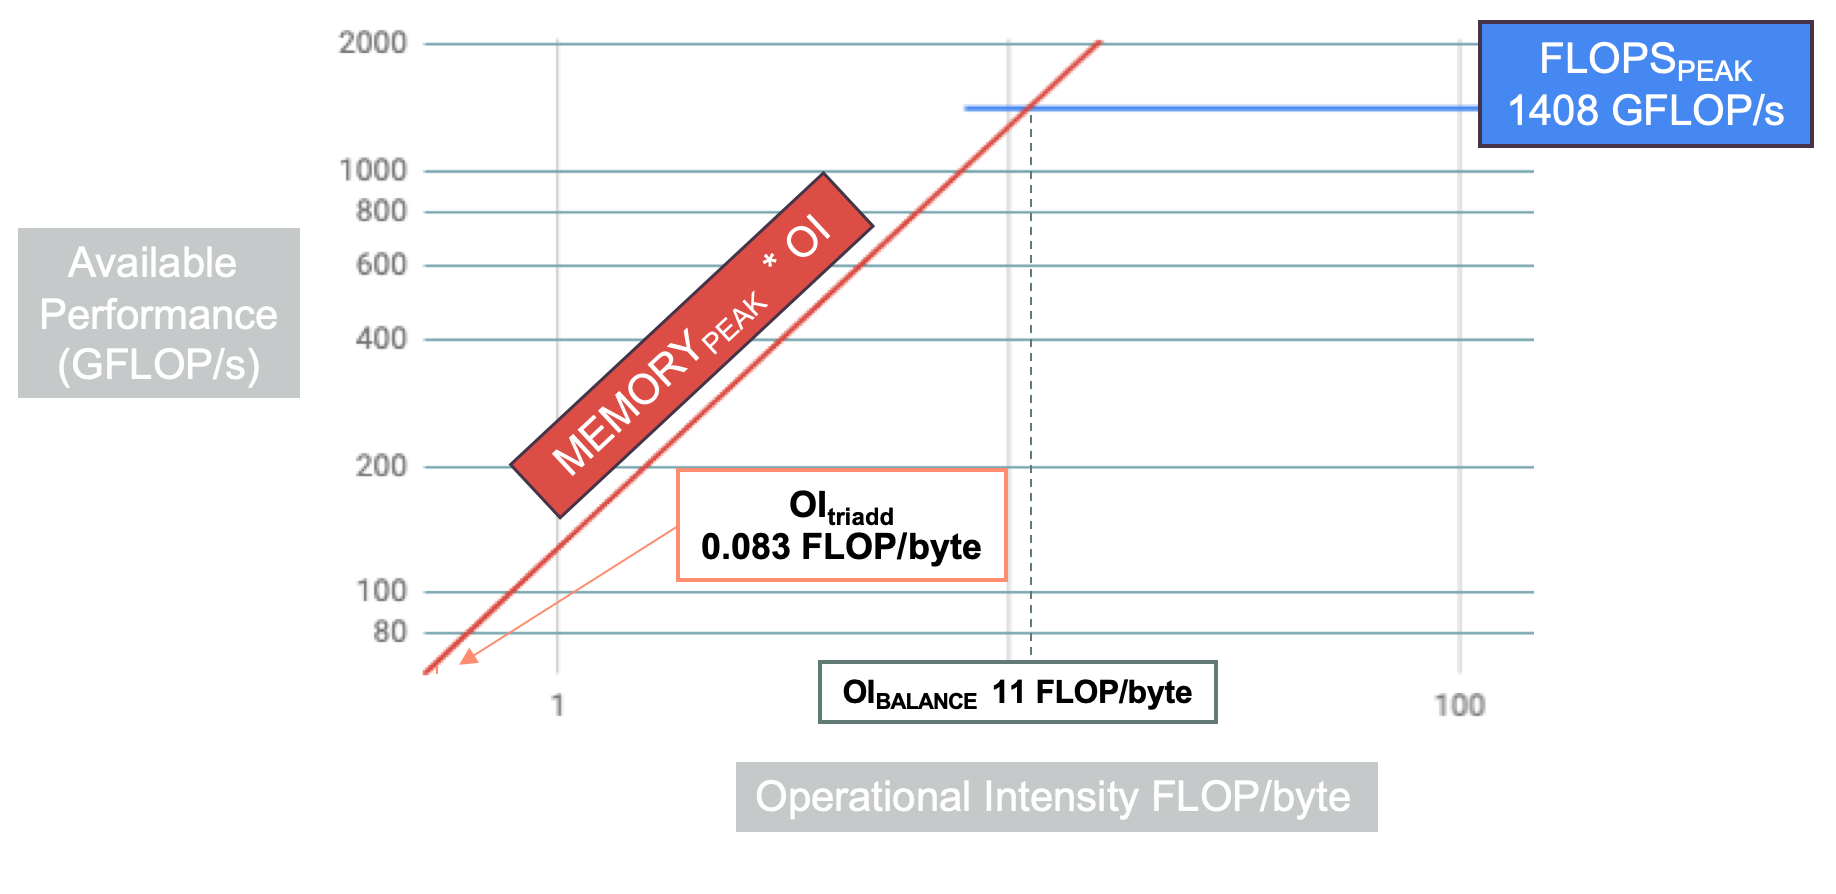
\includegraphics[width=14cm]{images/roofline_stream.png}
            \caption{\label{pic:Roofline_stream} Modèle du \textit{Roofline} appliqué à la fonction \textit{triadd} du benchmark \textit{Stream} et un processeur Xeon Skylake 6148.}
        \end{figure}
    


\subsubsection{Simple Memory Model} 
%%%%%%%%%%%%%%%%%
    L'analyse du noyau avec le modèle du Roofline indique que sur l'architecture ciblée, la performance du code sera limitée par la performance de la bande passante.

    
    Une fois assuré que les performances de l'application sont limitées par le système mémoire, le Simple Memory Model peut être appliqué. Dans notre expérimentation, nous utilisons trois matrices de 19.6 GB ($3 \times 10^9 \times sizeof(double)$). Pour une exécution optimale, le bus mémoire devrait être utilisé pour charger une fois les deux matrices en lectures (matrices B et C)  et pour l'écriture de la matrice A. Le trafic mémoire total serait alors de 58.8 GB. En utilisant les résultats mesurés lors de l'étape 2, on peut estimer le temps optimal pour l'exécution de cette fonction: $\text{TEMPS}_{optimal} = \frac{58.8}{128} = 0.56$ seconde. Cette modélisation nous permet de projeter la performance optimale sur une architecture sans avoir à exécuter le code sur celle-ci. Ainsi, nous pouvons comparer cette valeur avec la performance de l'architecture actuellement utilisée. Ceci permet de quantifier le gain de performance et d'avoir un modèle de performance à vérifier lorsque le portage sera réalisé.